\chapter{Metodología}










En este capítulo se describe la metodología utilizada para el entrenamiento, integración y evaluación de los modelos 
de deep learning orientados a la detección de enfermedades en hojas de plantas mediante una aplicación móvil.
El objetivo metodológico principal fue construir un flujo experimental que permitiera comparar dos arquitecturas diferentes 
de redes neuronales convolucionales, considerando no solo su desempeño predictivo, sino también su viabilidad de ejecución
en dispositivos móviles con recursos limitados. \\
La investigación se estructuró en distintas etapas: selección y preparación del conjunto de datos, 
entrenamiento de modelos de clasificación de imágenes, conversión de los modelos a un formato compatible con dispositivos Android, 
diseño de la interfaz de usuario para la aplicación móvil, desarrollo de la aplicación, integración de los modelos en la aplicación
móvil y evaluación experimental en condiciones controladas y reales. Esta metodologìa permitió analizar el comportamiento de los
modelos tanto en el entorno de desarrollo como en el dispositivo objetivo, manteniendo trazabilidad sobre las decisiones tomadas 
durante el proceso.



\section{Conjunto de datos}

Para el entrenamiento de los modelos se utilizó el conjunto de datos público PlantVillage \cite{DBLP:journals/corr/HughesS15},
ampliamente empleado en investigaciones relacionadas con la detección automática de enfermedades en plantas \cite{tembhurne2023plant24}. Este conjunto de datos
incluye 54.309 imágenes organizadas en 38 clases, correspondientes a hojas sanas y enfermas de 14 cultivos, manzana, arándano, cereza,
maíz, uva, naranja, melocotón, pimiento, patata, frambuesa, soja, calabaza, fresa y tomate. Se caracteriza por contar
con imágenes bien etiquetadas y de alta calidad, lo que permite construir un escenario de clasificación multiclase para evaluar el
desempeño de los modelos en un problema representativo a nivel investigativo.

En este estudio se utilizó el conjunto completo de cultivos disponibles. La selección de PlantVillage se fundamentó en su amplio uso
en la literatura científica, lo que favorece la comparabilidad y reproducibilidad de los resultados. Además, el conjunto de datos
incluye cultivos de alta relevancia productiva en Argentina, como soja y maíz. Dado que el objetivo de la investigación es evaluar la
viabilidad técnica y el desempeño en dispositivo móvil de arquitecturas ligeras de aprendizaje profundo, el enfoque adoptado es
independiente del cultivo particular y puede extenderse metodológicamente a otros contextos agrícolas.

En la figura \ref{fig:plantvillage_examples} se presentan algunos ejemplos de imágenes pertenecientes al conjunto de datos. Estas
muestras permiten observar el tipo de entrada visual utilizada durante el entrenamiento, así como parte de la variedad de cultivos y enfermedades
incluidas en el problema de clasificación.

\begin{figure}[H]
    \centering
    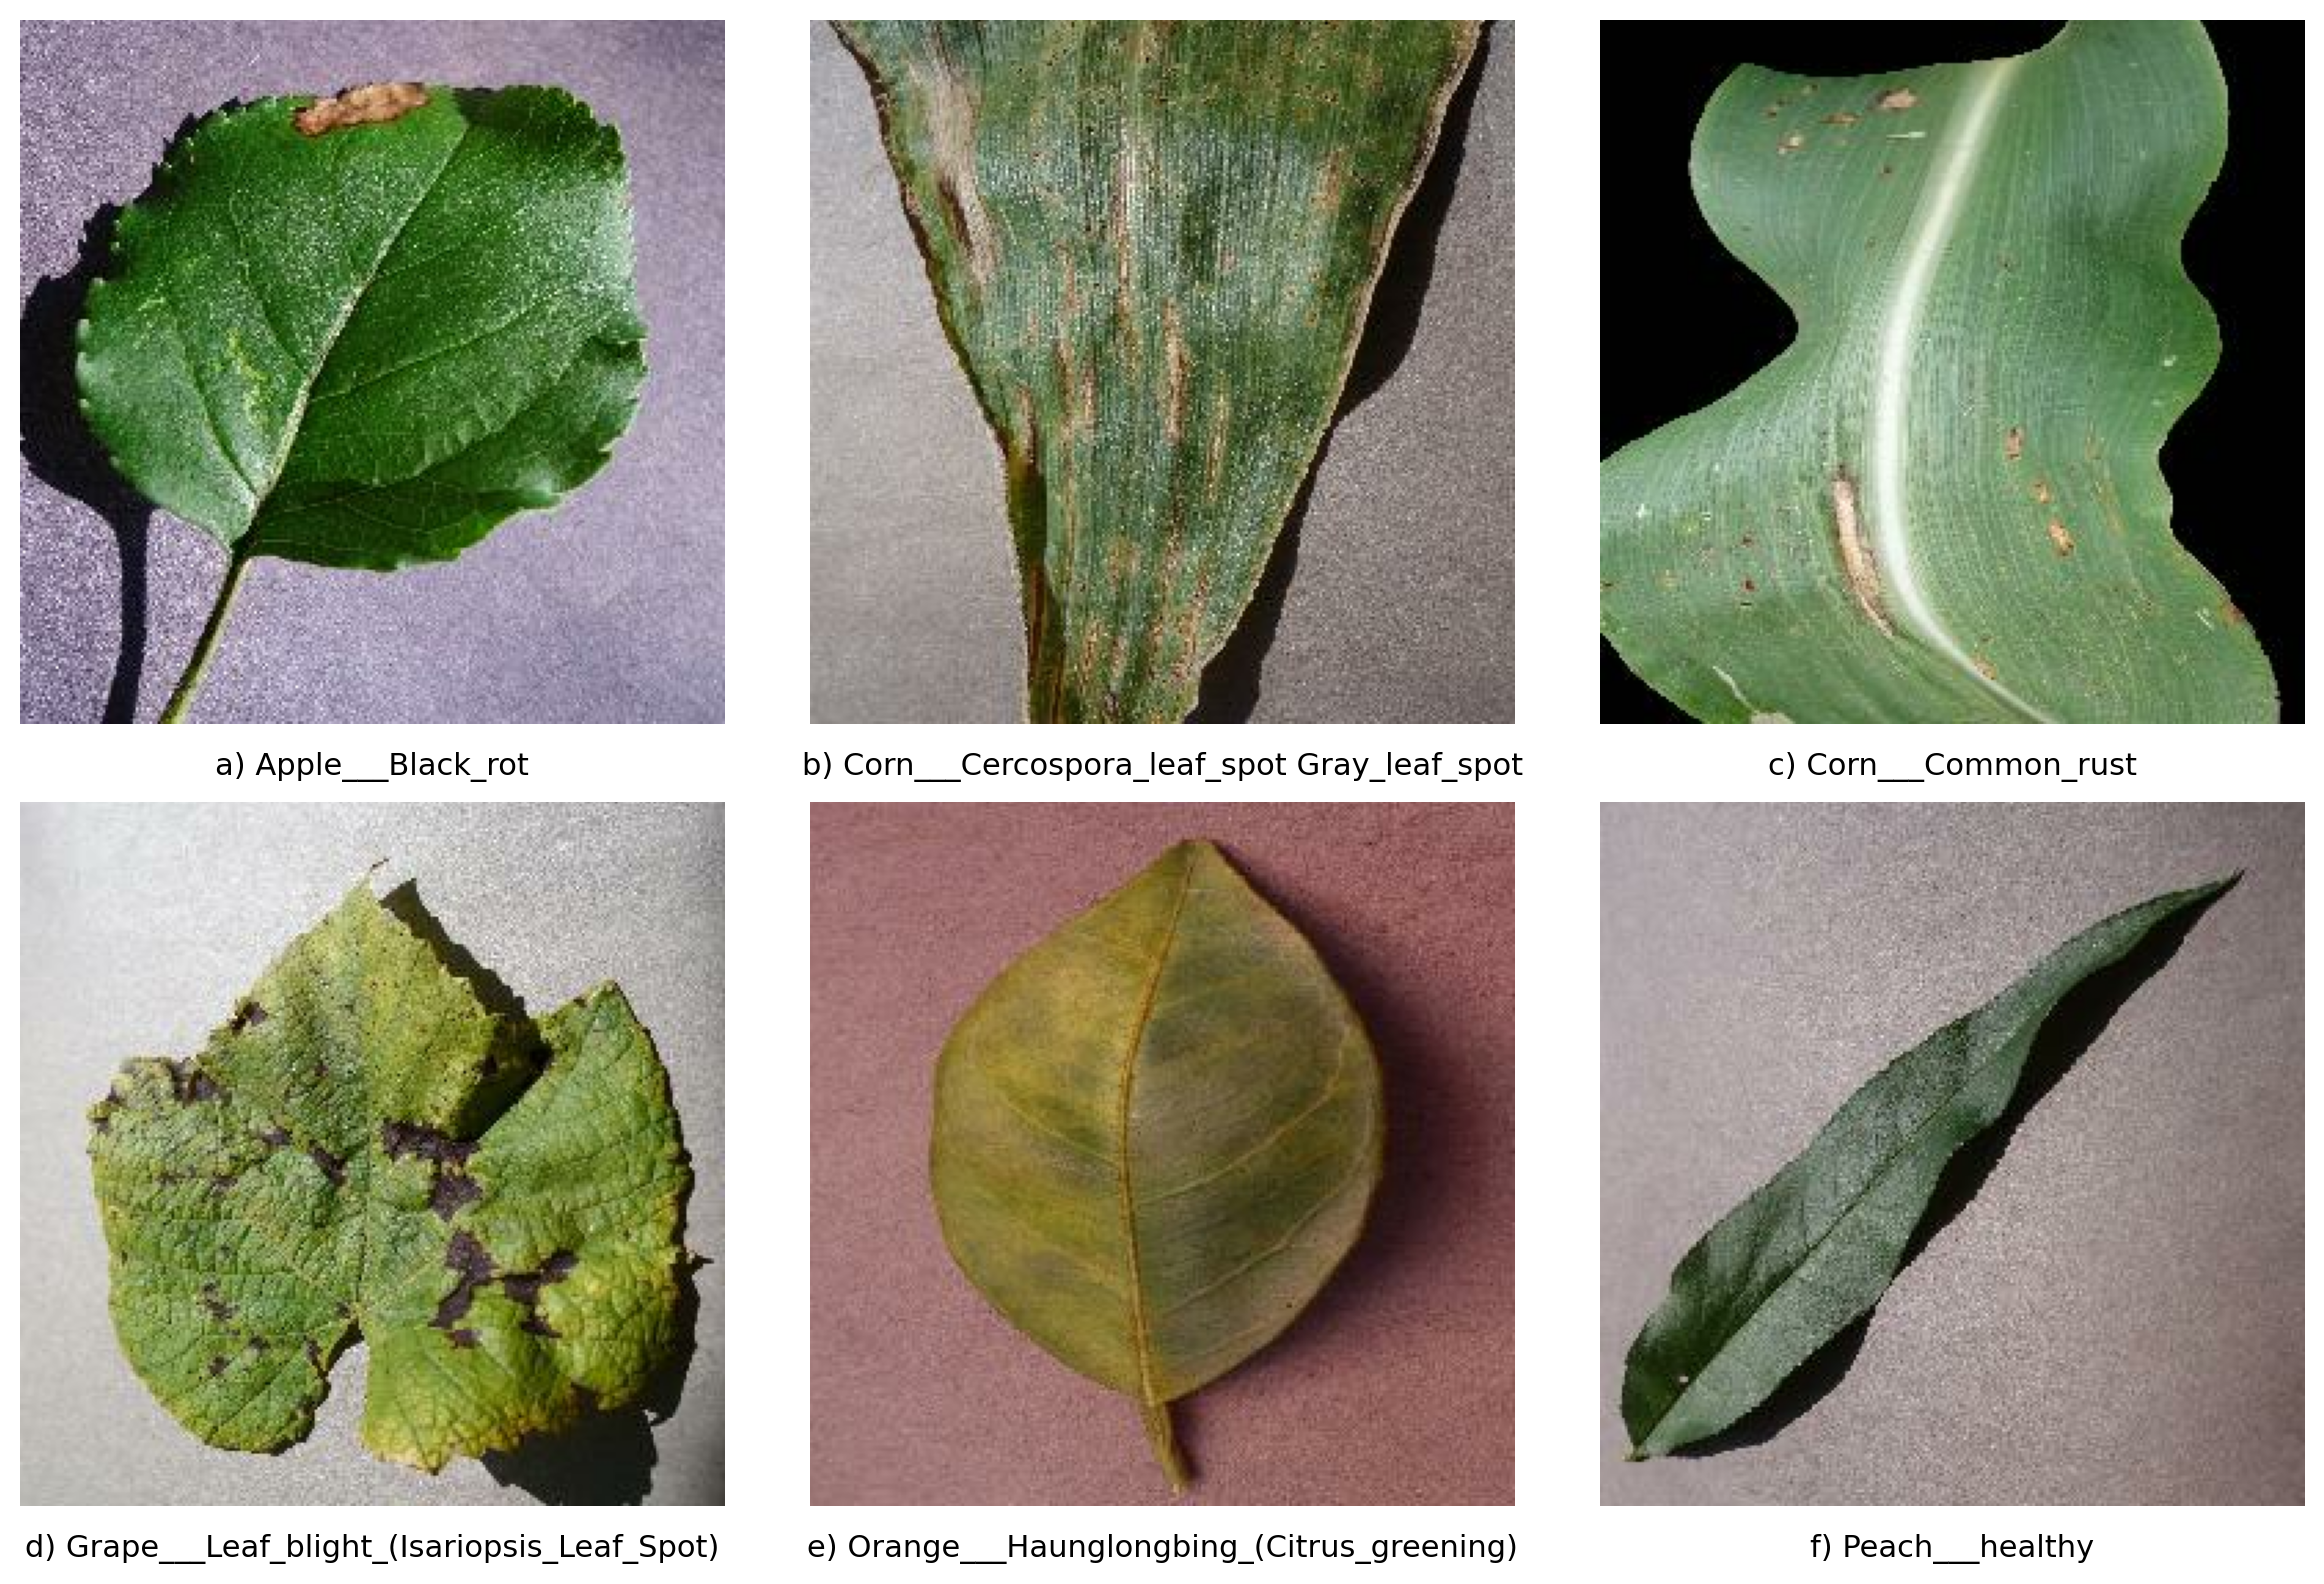
\includegraphics[width=1\textwidth]{images/ejemplos_plant_village.png}
    \caption{Ejemplos de imágenes del conjunto de datos PlantVillage: a) manzana con podredumbre negra, b) maíz con mancha foliar por Cercospora y mancha gris, c) maíz con roya común, d) uva con tizón foliar por Isariopsis, e) naranja con Huanglongbing o enverdecimiento de los cítricos, y f) durazno saludable.}
    \label{fig:plantvillage_examples}
\end{figure}

La distribución de imágenes por clase se puede observar en la figura \ref{fig:dataset_distribution}. Esta distribución permite
identificar la cantidad de ejemplos disponibles para cada categoría y ayuda a interpretar el comportamiento de los modelos durante
la evaluación, especialmente en un escenario donde se comparan clases de distintos cultivos y enfermedades.

\begin{figure}[H]
    \centering
    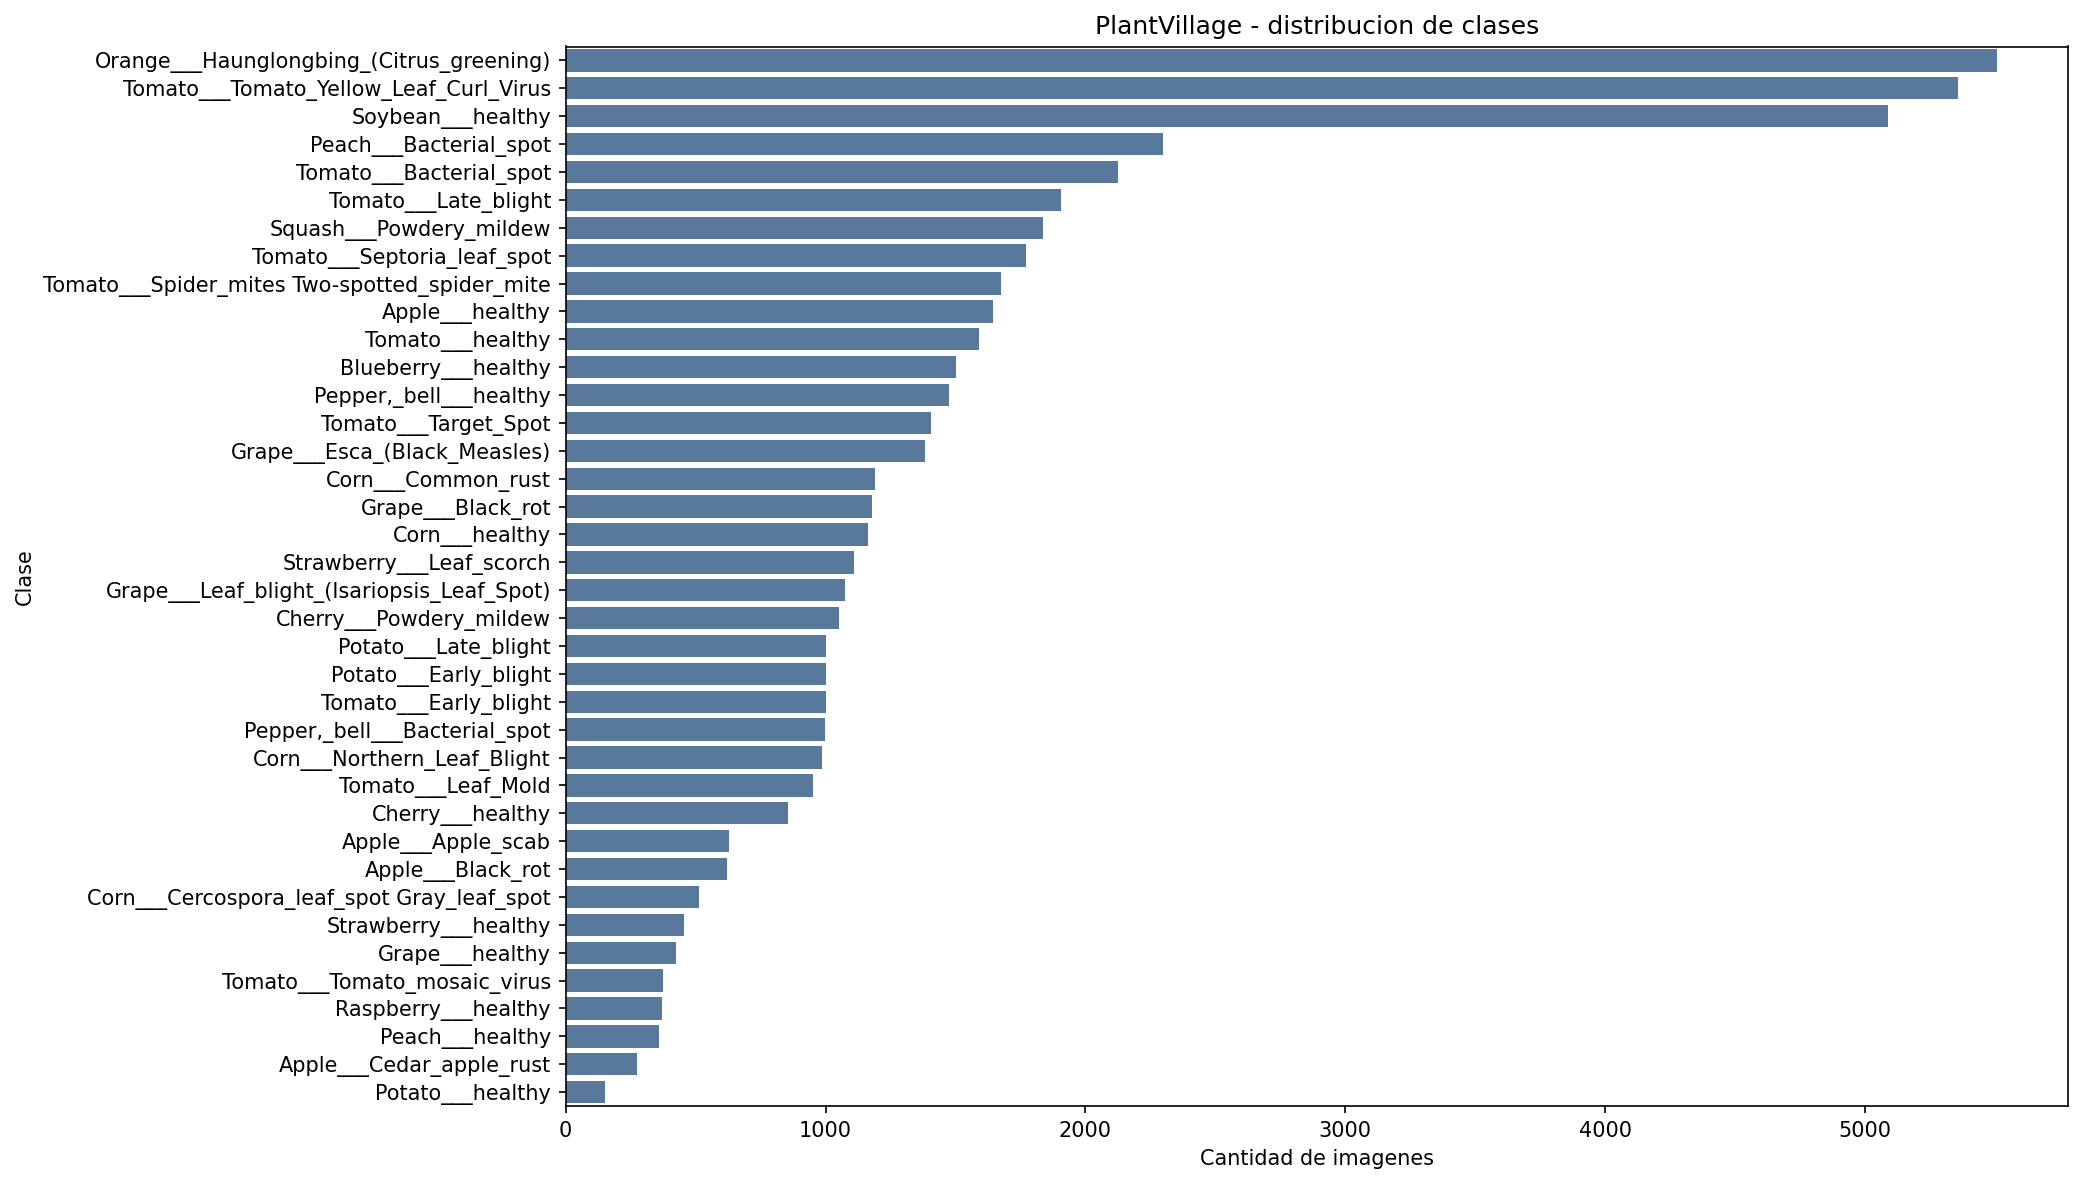
\includegraphics[width=1\textwidth]{images/dataset_distribution.png}
    \caption{Distribución del conjunto de datos PlantVillage por clase.}
    \label{fig:dataset_distribution}
\end{figure}

En la tabla \ref{tab:plantvillage_classes} se detallan las clases del conjunto de datos utilizadas en el entrenamiento, incluyendo
el cultivo, la enfermedad y el estado de salud de las plantas. Esta información es especialmente importante porque ayuda a comprender
la diversidad de casos que los modelos deben aprender a clasificar.


\begin{longtable}{>{\raggedright\arraybackslash}p{4.8cm}
                  >{\raggedright\arraybackslash}p{2.3cm}
                  >{\raggedright\arraybackslash}p{4.5cm}
                  >{\raggedright\arraybackslash}p{1.8cm}}
\caption{Clases del conjunto de datos PlantVillage utilizadas en el entrenamiento.}
\label{tab:plantvillage_classes}\\
\hline
\textbf{Clase} & \textbf{Cultivo} & \textbf{Enfermedad} & \textbf{Estado} \\
\hline
\endfirsthead
\hline
\textbf{Clase} & \textbf{Cultivo} & \textbf{Enfermedad} & \textbf{Estado} \\
\hline
\endhead
\path{Apple___Apple_scab} & Manzana & Sarna del manzano & Enferma \\
\path{Apple___Black_rot} & Manzana & Podredumbre negra & Enferma \\
\path{Apple___Cedar_apple_rust} & Manzana & Roya del cedro del manzano & Enferma \\
\path{Apple___healthy} & Manzana & Saludable & Saludable \\
\path{Blueberry___healthy} & Arándano & Saludable & Saludable \\
\path{Cherry___healthy} & Cereza & Saludable & Saludable \\
\path{Cherry___Powdery_mildew} & Cereza & Oídio & Enferma \\
\path{Corn___Cercospora_leaf_spot Gray_leaf_spot} & Maíz & Mancha foliar por Cercospora y mancha gris & Enferma \\
\path{Corn___Common_rust} & Maíz & Roya común & Enferma \\
\path{Corn___healthy} & Maíz & Saludable & Saludable \\
\path{Corn___Northern_Leaf_Blight} & Maíz & Tizón foliar del norte & Enferma \\
\path{Grape___Black_rot} & Uva & Podredumbre negra & Enferma \\
\path{Grape___Esca_(Black_Measles)} & Uva & Esca o sarampión negro & Enferma \\
\path{Grape___healthy} & Uva & Saludable & Saludable \\
\path{Grape___Leaf_blight_(Isariopsis_Leaf_Spot)} & Uva & Tizón foliar por Isariopsis & Enferma \\
\path{Orange___Haunglongbing_(Citrus_greening)} & Naranja & Huanglongbing o enverdecimiento de los cítricos & Enferma \\
\path{Peach___Bacterial_spot} & Durazno & Mancha bacteriana & Enferma \\
\path{Peach___healthy} & Durazno & Saludable & Saludable \\
\path{Pepper,_bell___Bacterial_spot} & Pimiento morrón & Mancha bacteriana & Enferma \\
\path{Pepper,_bell___healthy} & Pimiento morrón & Saludable & Saludable \\
\path{Potato___Early_blight} & Papa & Tizón temprano & Enferma \\
\path{Potato___healthy} & Papa & Saludable & Saludable \\
\path{Potato___Late_blight} & Papa & Tizón tardío & Enferma \\
\path{Raspberry___healthy} & Frambuesa & Saludable & Saludable \\
\path{Soybean___healthy} & Soja & Saludable & Saludable \\
\path{Squash___Powdery_mildew} & Calabaza & Oídio & Enferma \\
\path{Strawberry___healthy} & Frutilla & Saludable & Saludable \\
\path{Strawberry___Leaf_scorch} & Frutilla & Quemadura foliar & Enferma \\
\path{Tomato___Bacterial_spot} & Tomate & Mancha bacteriana & Enferma \\
\path{Tomato___Early_blight} & Tomate & Tizón temprano & Enferma \\
\path{Tomato___healthy} & Tomate & Saludable & Saludable \\
\path{Tomato___Late_blight} & Tomate & Tizón tardío & Enferma \\
\path{Tomato___Leaf_Mold} & Tomate & Moho foliar & Enferma \\
\path{Tomato___Septoria_leaf_spot} & Tomate & Mancha foliar por Septoria & Enferma \\
\path{Tomato___Spider_mites Two-spotted_spider_mite} & Tomate & Ácaro de dos manchas & Enferma \\
\path{Tomato___Target_Spot} & Tomate & Mancha objetivo & Enferma \\
\path{Tomato___Tomato_mosaic_virus} & Tomate & Virus del mosaico del tomate & Enferma \\
\path{Tomato___Tomato_Yellow_Leaf_Curl_Virus} & Tomate & Virus del rizado amarillo de la hoja del tomate & Enferma \\
\hline
\end{longtable}

Es importante destacar que, aunque PlantVillage es un recurso valioso para el entrenamiento de modelos, su uso también presenta
desafíos. Las imágenes del conjunto de datos no necesariamente reflejan por completo las condiciones reales de un cultivo, donde pueden
existir variaciones de iluminación, fondos más complejos y presencia de otras plantas o elementos. Por esta razón, se incluyeron
imágenes de fondo aleatorio sin hojas (IFD) durante la evaluación en dispositivo móvil, con el fin de observar cómo los modelos
responden a entradas fuera del dominio esperado. Esta estrategia permitió evaluar la robustez de los modelos frente a situaciones del
mundo real que podrían no estar representadas en el conjunto de datos original.


\section{Modelos de aprendizaje profundo}
Durante el proceso de investigación se encontraron en la literatura diversas arquitecturas utilizadas para la clasificación
de imágenes. Dentro de estas, las redes neuronales convolucionales o CNN (Convolutional Neural Networks) han demostrado un alto
rendimiento en tareas como clasificación, detección y segmentación de imágenes. Esto se debe a su capacidad para extraer patrones
visuales relevantes a partir de filtros entrenables, aprendiendo características como bordes, texturas, formas y combinaciones más
complejas a medida que aumenta la profundidad de la red.

En el contexto agrícola, distintos trabajos han utilizado modelos basados en CNN para la detección automática de enfermedades en hojas.
Por ejemplo, \cite{agronomy13040961} evaluó más de 15 modelos preentrenados, incluyendo arquitecturas como ResNet, EfficientNet y
MobileNetV2, para el reconocimiento de enfermedades en hojas de arroz, obteniendo precisiones superiores al 97\% en todos los casos.
De manera similar, \cite{subramaniam2026comparative} realizó un trabajo comparativo de modelos de aprendizaje profundo para la
detección de enfermedades en cultivos, donde el modelo EfficientNet alcanzó el mejor desempeño con una exactitud de 97,4\%.

Sin embargo, dado que el objetivo de esta investigación es desarrollar una solución viable para dispositivos móviles, la precisión no
es el único criterio de selección. También es necesario considerar la eficiencia computacional, el tamaño del modelo, el tiempo de
inferencia y la posibilidad de ejecutar la predicción directamente en el dispositivo. En este sentido, se consideró valiosa la
comparación entre modelos de la familia MobileNet, diseñados específicamente para trabajar con recursos limitados, y modelos de la
familia EfficientNet, que ofrecen un buen balance entre precisión y eficiencia, aunque pueden requerir una mayor cantidad de parámetros
dependiendo de la versión utilizada.

Desde el punto de vista metodológico, la comparación entre estas arquitecturas permite analizar no solo cuál modelo obtiene mejores
resultados en el entrenamiento, sino también cuál resulta más adecuado para integrarse en una aplicación móvil. Por esta razón, la
evaluación se realizó considerando tanto métricas de clasificación como aspectos prácticos de implementación, entre ellos el tiempo de
inferencia, el uso de memoria, la confianza de las predicciones y el comportamiento frente a imágenes que no contienen hojas.

\subsection{Modelos MobileNet}
MobileNet es una familia de arquitecturas de redes neuronales convolucionales desarrollada por Google y optimizada específicamente
para dispositivos móviles y sistemas embebidos \cite{howard2017mobilenetsefficientconvolutionalneural}. Su uso resulta adecuado para
esta investigación porque el objetivo no es solamente obtener una buena precisión durante el entrenamiento, sino también integrar el
modelo en una aplicación Android y ejecutarlo en un dispositivo con recursos limitados.

Dentro de la familia MobileNet se consideraron distintas versiones como parte del proceso experimental. MobileNetV2 funcionó como punto
de referencia inicial, ya que es una arquitectura ampliamente utilizada en aplicaciones móviles. Posteriormente se evaluó MobileNetV3,
que representa una evolución natural de esta familia y mantiene una arquitectura diseñada para dispositivos móviles, exportable a
TensorFlow Lite y metodológicamente coherente con el objetivo de la aplicación. MobileNetV5 se consideró como un experimento exploratorio,
pero el preset disponible en KerasHub resultó demasiado grande para una aplicación móvil común, por lo que no fue seleccionado como
modelo final.

MobileNetV3 fue diseñada para dispositivos móviles y de borde (edge), donde la capacidad de procesamiento suele ser limitada. Esta
versión prioriza la precisión, la eficiencia y la velocidad, incorporando bloques livianos que permiten reducir el costo computacional
durante la inferencia. Además, cuenta con dos variantes principales: MobileNetV3-Large y MobileNetV3-Small. La variante Small ofrece un
mejor equilibrio entre velocidad, tamaño y precisión para aplicaciones móviles, siendo su peso aproximadamente cuatro quintos del tamaño
de la versión Large \cite{li2022mobilenetv3}. Con base en estas características, la elección final de uno de los modeloa a utilizar en la aplicación
móvil fue MobileNetV3-Small.


\subsection{Modelos EfficientNet}
EfficientNet es una familia de redes neuronales convolucionales diseñada para mejorar la relación entre precisión y eficiencia
computacional \cite{tan2020efficientnetrethinkingmodelscaling}. A diferencia de otras arquitecturas que aumentan principalmente la
profundidad o el ancho de la red, EfficientNet propone un escalado compuesto, donde se ajustan de manera conjunta la profundidad, el
ancho y la resolución de entrada del modelo. Esta estrategia permite mejorar el rendimiento en tareas de clasificación de imágenes sin
incrementar innecesariamente el costo computacional.

En el año 2021 se introdujo EfficientNetV2, una evolución de la arquitectura original orientada a obtener modelos más pequeños y con
entrenamientos más rápidos \cite{DBLP:journals/corr/abs-2104-00298}. Esta versión incorpora cambios en la estructura de los bloques
convolucionales y mantiene el objetivo de lograr un buen equilibrio entre capacidad de representación, precisión y eficiencia. Dentro
de esta familia, EfficientNetV2B0 resulta una variante relevante que corresponde a una versión base y liviana, que ha demostrado
tener la buena precisión en comparación con otras arquitecturas como ResNet50 \cite{molcan2023classification}.

En el marco de esta investigación, EfficientNetV2B0 se incorporó como una alternativa de comparación frente a los modelos de la familia
MobileNet. Su inclusión permite analizar si una arquitectura con mayor capacidad de representación puede mejorar la clasificación de
enfermedades en hojas y, al mismo tiempo, evaluar el costo asociado en términos de tamaño del modelo, tiempo de inferencia y desempeño
en el dispositivo móvil utilizado para las pruebas. De esta manera, la comparación no se limita únicamente a la exactitud obtenida en
el entrenamiento, sino que también considera la viabilidad práctica del modelo dentro de una aplicación móvil.

\section{Aplicación en dispositivos móviles}
Para implementar los modelos de Deep Learning en dispositivos móviles, se utilizó TensorFlow Lite, una biblioteca de aprendizaje automático optimizada para dispositivos móviles. Se realizaron pruebas de rendimiento para evaluar la velocidad de inferencia y el consumo de recursos en diferentes dispositivos móviles, asegurando que los modelos sean viables para su uso en tiempo real en el reconocimiento de enfermedades en plantas. Además, se desarrolló una aplicación móvil que integra los modelos entrenados, permitiendo a los usuarios capturar imágenes de plantas y recibir diagnósticos instantáneos sobre posibles enfermedades presentes.


\subsection{Desarrollo de la aplicación móvil}

Un aspecto relevante de la metodología fue la evaluación en dispositivo móvil, utilizando un teléfono Moto G como entorno de prueba. Esta etapa permitió medir el desempeño real de los modelos luego de su integración en la aplicación, más allá de los resultados obtenidos en notebooks de entrenamiento. Asimismo, se incluyeron imágenes de fondo aleatorio sin hojas, denominadas IFD, con el fin de observar la respuesta de los modelos ante entradas fuera del dominio esperado.

\subsection{Implementación de la interfaz de usuario}
La interfaz de usuario de la aplicación móvil fue diseñada para ser intuitiva y fácil de usar, permitiendo a los usuarios capturar imágenes de plantas y recibir diagnósticos de manera rápida y eficiente. Se implementaron funcionalidades adicionales, como la visualización de resultados históricos y recomendaciones para el cuidado de las plantas, basadas en los diagnósticos obtenidos por los modelos de Deep Learning.

\subsection{Implmentación de los modelos de Deep Learning en la aplicación móvil}
Los modelos de Deep Learning entrenados fueron convertidos a un formato compatible con TensorFlow Lite para su implementación en la aplicación móvil. Se realizaron pruebas exhaustivas para asegurar que los modelos funcionen correctamente en diferentes dispositivos móviles, evaluando tanto la precisión de las predicciones como el rendimiento en términos de velocidad de inferencia y consumo de recursos. Se optimizó el código para garantizar una experiencia de usuario fluida y eficiente, permitiendo a los usuarios obtener diagnósticos en tiempo real sobre las enfermedades presentes en sus plantas.

\subsection{Captura de imágenes y diagnóstico en tiempo real}

\subsection{Obtención de resultados y análisis de desempeño}
